\chapter*{GPT-3 : Part 1 - The Transformer}
\label{chap:transformer}
\thispagestyle{fancy}
\addcontentsline{toc}{chapter}{\nameref{chap:transformer}}

\hspace{0.5cm} Introduced in 2017, The Transformer is a deep learning model primarily used in the field of natural language processing (NLP). Transformers are designed to handle sequential data, such as natural language unlike RNNs, Transformers do not require that the sequential data be processed in order. Thus Transformer allows for much more parallelization than RNNs and therefore reduced training hours. This has led to the development of pre-trained systems such as BERT (Bidirectional Encoder Representations from Transformers) and GPT (Generative Pre-trained Transformer), which have been trained with huge general language datasets, and can be fine-tuned to specific language tasks.

Transformer is an encoder-decoder architecture. The \emph{encoder} consists of a set of encoding layers that processes the input iteratively one layer after another and the \emph{decoder} consists of a set of decoding layers that does the same thing to the output of the encoder. Each encoder and decoder layer makes use of an \emph{attention mechanism}, which for each input, weighs the relevance of every other input and draws information from them accordingly to produce the output. Each decoder layer also has an additional attention mechanism which draws information from the outputs of previous decoders, before the decoder layer draws information from the encodings. Both the encoder and decoder layers have a feed-forward neural network for additional processing of the outputs, and contain residual connections and layer normalization steps \cite{wiki:transformer} as shown in figure \ref{fig:trnsfrmarch}.

\begin{figure}[!htbp]
    \centering
    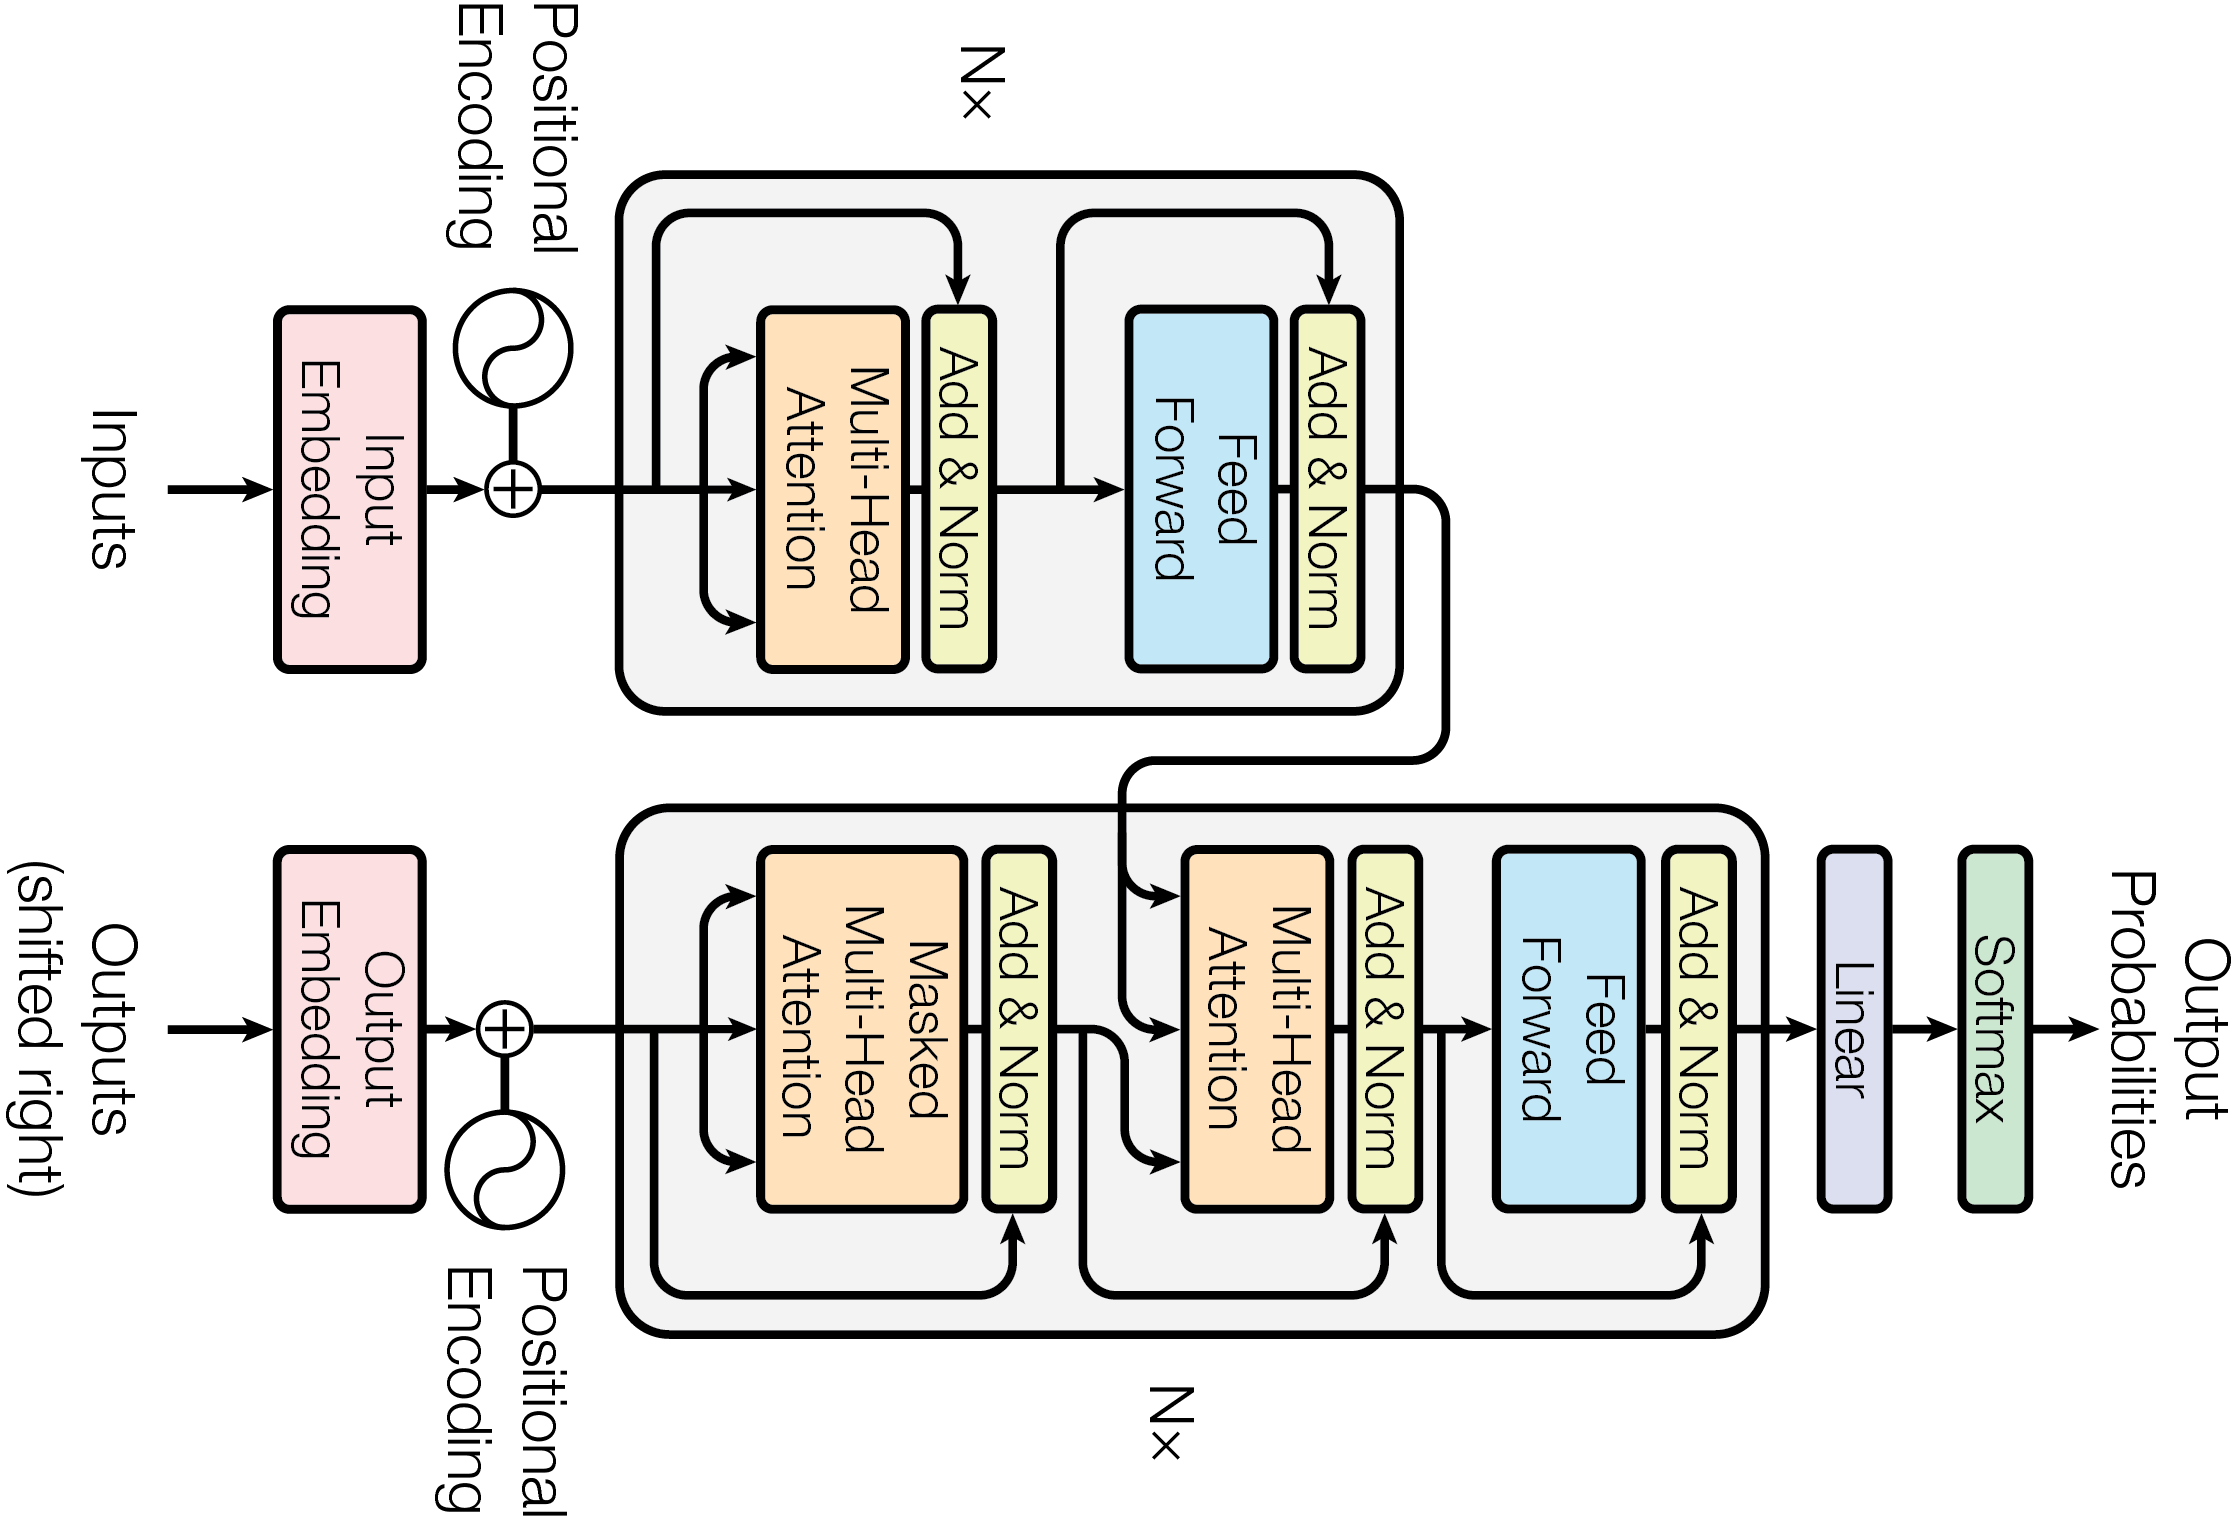
\includegraphics[width=0.7\textwidth]{transformer.png}
    \caption[The Transformer - model architecture]{The Transformer - model architecture \cite{2017arXiv170603762V}}
    \label{fig:trnsfrmarch}
\end{figure}

The basic building blocks of the Transformer are scaled dot-product attention units. When a sentence is passed into a Transformer model, attention weights are calculated between every token simultaneously. The attention unit produces embeddings for every token in context that contain information not only about the token itself, but also a weighted combination of other relevant tokens weighted by the attention weights.

\section*{Encoder}
\label{sec:encdr}
\addcontentsline{toc}{section}{\nameref{sec:encdr}}

\hspace{0.5cm} The encoder is composed of a stack of $N = 6$ identical layers. Each layer has two sub-layers. The first is a multi-head self-attention mechanism, and the second is a simple, position-wise fully connected feed-forward network. A residual connection \cite{2016arXiv160202410J} around each of the two sub-layers, followed by layer normalization \cite{2016arXiv160706450L}. That is, the output of each sub-layer is $LayerNorm(x + Sublayer(x))$, where $Sublayer(x)$ is the function implemented by the sub-layer itself \cite{2017arXiv170603762V}.

\section*{Decoder}
\label{sec:decdr}
\addcontentsline{toc}{section}{\nameref{sec:decdr}}

\hspace{0.5cm} The decoder is also composed of a stack of $N = 6$ identical layers. In addition to the two sub-layers in each encoder layer, the decoder inserts a third sub-layer, which performs multi-head attention over the output of the encoder stack. Similar to the encoder, residual connections are employed around each of the sub-layers, followed by layer normalization. The self-attention sublayer is also modified in the decoder stack to prevent positions from attending to subsequent positions. This masking, combined with fact that the output embeddings are offset by one position, ensures that the predictions for position $i$ can depend only on the known outputs at positions less than $i$ \cite{2017arXiv170603762V}.

\section*{Attention Mechanism}
\label{sec:attnmec}
\addcontentsline{toc}{section}{\nameref{sec:attnmec}}

\begin{figure}[!htbp]
    \centering
    \begin{minipage}{0.45\textwidth}
        \centering
        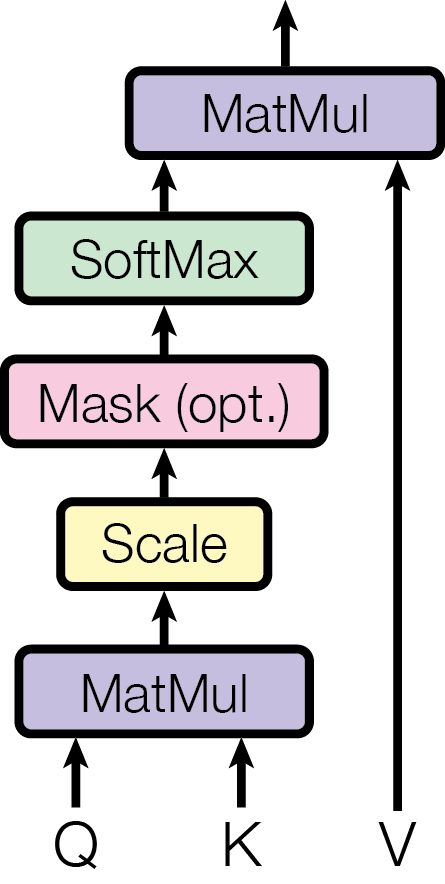
\includegraphics[height=0.7\textwidth]{scaled_dot_attention.png}
        \caption[Scaled Dot-Product Attention]{\centering Scaled Dot-Product Attention \cite{2017arXiv170603762V}}
        \label{fig:sdpa}
    \end{minipage}\hfill
    \begin{minipage}{0.45\textwidth}
        \centering
        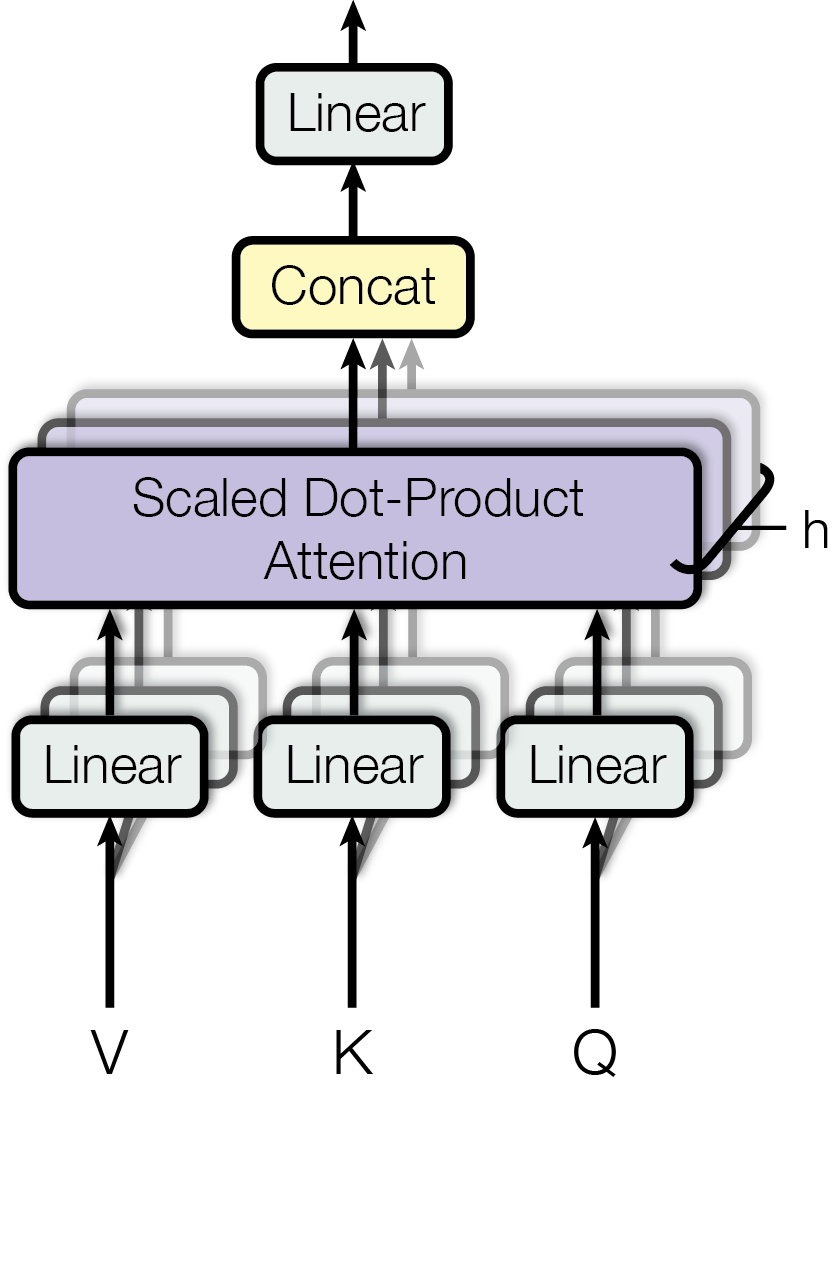
\includegraphics[height=0.7\textwidth]{masked_multihead_attention.png}
        \caption[Masked Multi-head Attention]{\centering Masked Multi-head Attention \cite{2017arXiv170603762V}}
        \label{fig:mmha}
    \end{minipage}
\end{figure}

\hspace{0.5cm} An attention function can be described as mapping a query and a set of key-value pairs to an output, where the query, keys, values, and output are all vectors. The output is computed as a weighted sum of the values, where the weight assigned to each value is computed by a compatibility function of the query with the corresponding key.

The input consists of queries and keys of dimension $d_k$, and values of dimension $d_v$. The dot products of the query with all keys is computed then each one divided by $\sqrt{d_k}$. Finally a \emph{softmax} function is applied to obtain the weights on the values. In practice, the attention function on a set of queries is computed simultaneously, packed together into a matrix $Q$. The keys and values are also packed together into matrices $K$ and $V$ as shown in figures \eqref{fig:sdpa} and \eqref{fig:mmha}. The matrix of outputs is computed as \cite{2017arXiv170603762V}:

\[\textnormal{Attention}(Q, K, V) = \textnormal{softmax}(\frac{(Q K^T)}{\sqrt{d_k}})V\]


\vspace*{\fill}